		% --------------------------------------------------------------
% This is all preamble stuff that you don't have to worry about.
% Head down to where it says "Start here"
% --------------------------------------------------------------
 
\documentclass[12pt]{article}
 
\usepackage[margin=1in]{geometry} 
\usepackage{amsmath,amsthm,amssymb}
\usepackage{graphicx}
\usepackage{subcaption}
\usepackage{listings}
\usepackage{hyperref}
\usepackage{color}
%\usepackage{algorithm,algorithmic}
\usepackage{mathtools}


\newcommand{\argmax}{\arg\!\max}
\definecolor{codegreen}{rgb}{0,0.6,0}
\definecolor{codegray}{rgb}{0.5,0.5,0.5}
\definecolor{codepurple}{rgb}{0.58,0,0.82}
\definecolor{backcolour}{rgb}{0.95,0.95,0.92}

\lstdefinestyle{mystyle}{
	backgroundcolor=\color{backcolour},   
	commentstyle=\color{codegreen},
	keywordstyle=\color{magenta},
	numberstyle=\tiny\color{codegray},
	stringstyle=\color{codepurple},
	basicstyle=\footnotesize,
	breakatwhitespace=false,         
	breaklines=true,                 
	captionpos=b,                    
	keepspaces=true,                 
	numbers=left,                    
	numbersep=5pt,                  
	showspaces=false,                
	showstringspaces=false,
	showtabs=false,                  
	tabsize=2
}

\lstset{style=mystyle}

\newcommand{\N}{\mathbb{N}}
\newcommand{\Z}{\mathbb{Z}}

\newenvironment{problem}[2][\large Problem]{\begin{trivlist}
\item[\hskip \labelsep {\bfseries #1}\hskip \labelsep {\bfseries #2.}]}{\end{trivlist}}
 
\newenvironment{theorem}[2][Theorem]{\begin{trivlist}
\item[\hskip \labelsep {\bfseries #1}\hskip \labelsep {\bfseries #2.}]}{\end{trivlist}}

\newenvironment{ack}[2][Acknowledgements]{\begin{trivlist}
\item[\hskip \labelsep {\bfseries #1}\hskip \labelsep {\bfseries #2}]}{\end{trivlist}}


\renewcommand\section{\@startsection{section}{1}{\z@}%
                       {-1.2ex \@plus -0.8ex \@minus -0.8ex}%
                       {0.8ex \@plus 0.4ex \@minus 0.4ex}%
                       {\normalfont\large\bfseries\boldmath
                        \rightskip=\z@ \@plus 8em\pretolerance=10000 }}
\renewcommand\subsection{\@startsection{subsection}{2}{\z@}%
                       {-1.0ex \@plus -0.6ex \@minus -0.6ex}%
                       {1.0ex \@plus 0.3ex \@minus 0.3ex}%
                       {\normalfont\normalsize\bfseries\boldmath
                        \rightskip=\z@ \@plus 8em\pretolerance=10000 }}

\makeatother   % Cancel the effect of \makeatletter


\setlength{\parindent}{0in}
\setlength{\parskip}{1ex}
\begin{document}
 
% --------------------------------------------------------------
%                         Start here
% --------------------------------------------------------------
 
%\renewcommand{\qedsymbol}{\filledbox}
 
\title{EECS 598: Reinforcement Learning, Homework 2}%replace X with the appropriate number
\author{Abhishek Venkataraman} %if necessary, replace with your course title
 
\maketitle
 
\begin{problem} {1} Stochastic Dyna-Q
\\
In order to account for stochasticity, :

Converged policy for Dyna-Q:
$$ Policy = \begin{bmatrix} 
 0.,  0.,  0.,  1.\\
 0.,  0.,  0.,  1.\\
 0.,  0.,  0.,  1.\\
 0.,  0.,  1.,  0.\\
 0.,  1.,  0.,  0.\\
 1.,  0.,  0.,  0.\\
 1.,  0.,  0.,  0.\\
 1.,  0.,  0.,  0.\\
 1.,  0.,  0.,  0.\\
 0.,  0.,  1.,  0.\\
 0.,  0.,  0.,  1.\\
 0.,  0.,  0.,  1.\\
 0.,  1.,  0.,  0.\\
 0.,  1.,  0.,  0.\\
 0.,  1.,  0.,  0.\\
 1.,  0.,  0.,  0.\\
 1.,  0.,  0.,  0.\\
 1.,  0.,  0.,  0.\\
 0.,  1.,  0.,  0.\\
 0.,  0.,  1.,  0.\\
 0.,  1.,  0.,  0.\\
 0.,  1.,  0.,  0.\\
 0.,  1.,  0.,  0.\\
 1.,  0.,  0.,  0.\\
\end{bmatrix} $$ 
Parameters: $\#episodes = 400$, $\#planning = 50$, $\epsilon = 0.02$,
$\alpha = 0.1$, $\gamma = 0.99$, $\kappa = None$

Reasons:
\vspace{-4mm} 
\begin{itemize}
	\item I was not able to reach the goal state many times in just 30 episodes
	\item I changed the number of planning steps but that did not affect the results much
	\item Large $\epsilon$ leads to more random action. Given that the environment has a large number of holes, it is essential that the optimal action is taken more often. Hence $\epsilon$ small value lets the cumulative reward increase.
	\item I used the default learning rate. It did not affect the policy convergence a lot
	\item since the reward is small and a lot of time, the agent falls into hole, I increased $\gamma$ so that the goal state helps the agent to be directed towards it 
\end{itemize}

Converged policy for Dyna-Q+:
$$ Policy = \begin{bmatrix} 
 0.,  0.,  0.,  1.\\
 0.,  0.,  0.,  1.\\
 0.,  0.,  0.,  1.\\
 0.,  0.,  1.,  0.\\
 1.,  0.,  0.,  0.\\
 1.,  0.,  0.,  0.\\
 1.,  0.,  0.,  0.\\
 1.,  0.,  0.,  0.\\
 1.,  0.,  0.,  0.\\
 0.,  0.,  1.,  0.\\
 0.,  0.,  0.,  1.\\
 0.,  0.,  0.,  1.\\
 0.,  1.,  0.,  0.\\
 0.,  1.,  0.,  0.\\
 0.,  1.,  0.,  0.\\
 1.,  0.,  0.,  0.\\
 1.,  0.,  0.,  0.\\
 1.,  0.,  0.,  0.\\
 0.,  0.,  0.,  1.\\
 0.,  0.,  1.,  0.\\
 0.,  1.,  0.,  0.\\
 0.,  1.,  0.,  0.\\
 0.,  1.,  0.,  0.\\
 1.,  0.,  0.,  0.\\
\end{bmatrix} $$ 
Parameters: $\#episodes = 400$, $\#planning = 50$, $\epsilon = 0.02$,
$\alpha = 0.1$, $\gamma = 0.99$, $\kappa = 0.0001$

Reason: A large kappa was priority gives preference for visiting non goals states over goal state. This reduces the overall cumulative reward. The other parameters were the same as Dyna-Q method. 



\end{problem}
\newpage

\begin{problem} {2} Dyna-Q vs. Dyna-Q+\\
\begin{figure}[h]
	\centering
	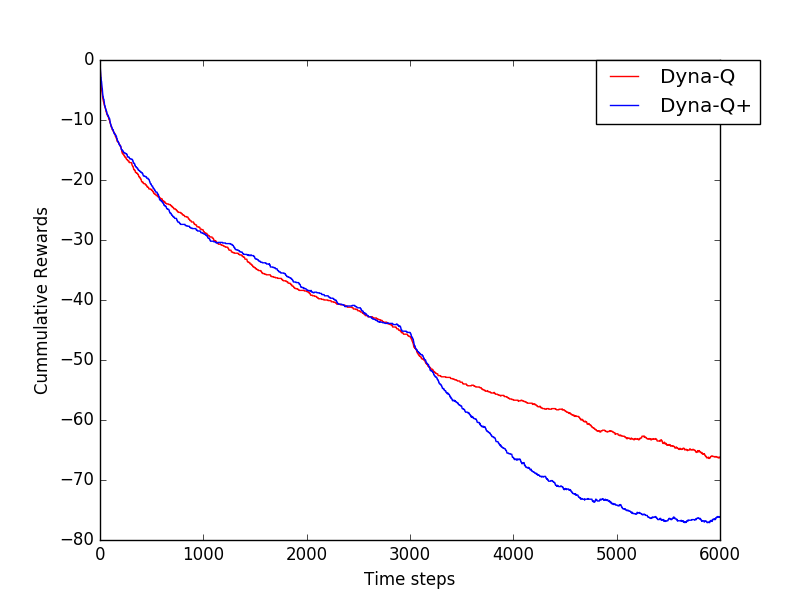
\includegraphics[width = 0.9\linewidth]{prob2_10agents.png}
\end{figure}	
\end{problem}
%\newpage
\begin{problem} {3} Prioritized Sweeping\\
\begin{figure}[h]
	\centering
	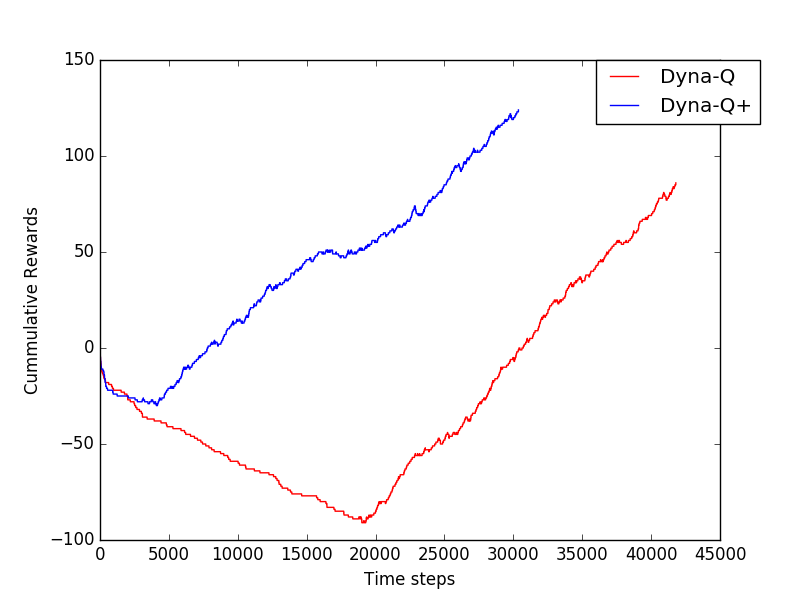
\includegraphics[width = 0.45\linewidth]{DQ_DQ_plus.png}
	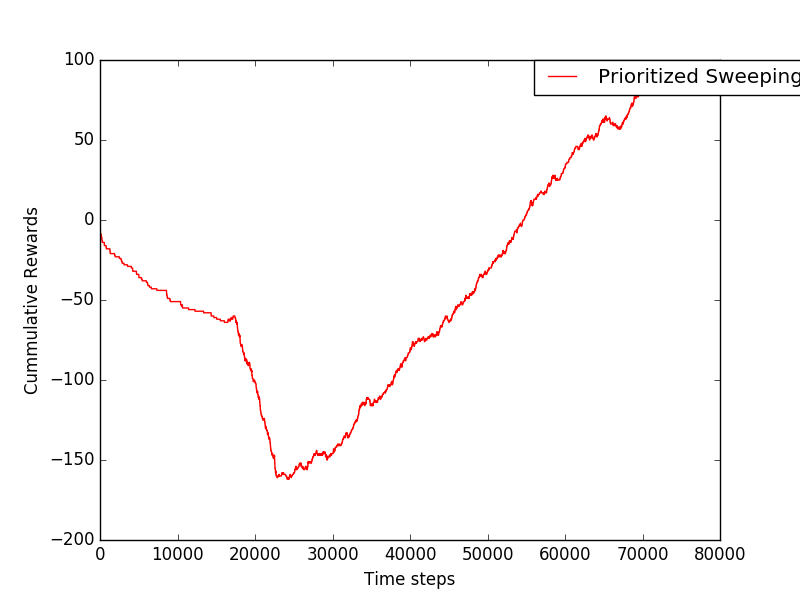
\includegraphics[width = 0.45\linewidth]{PS.png}
\end{figure}	
Prioritized Sweeping seems to be converging slower than Dyna-Q and Dyna-Q+. I suspect that this is highly dependent on the parameters chosen. In case of Dyna-Q/Q+ the num of planning episodes was 50 while in case of this, the number of planning step was only 20. I suspect that this is a main reason for the difference. 
\newpage

Policy obtained by Prioritized Sweeping with the following parameters:\\ \#episodes= 1000, \#planning= 20, $ \epsilon = 0.02$, $\alpha = 0.1$, $\gamma = 0.99 $, $\theta = 0.5$
$$ Policy = \begin{bmatrix} 
 0. & 0. & 0. & 1.\\
 0. & 0. & 0. & 1.\\
 0. & 0. & 0. & 1.\\
 0. & 0. & 1. & 0.\\
 1. & 0. & 0. & 0.\\
 1. & 0. & 0. & 0.\\
 1. & 0. & 0. & 0.\\
 1. & 0. & 0. & 0.\\
 1. & 0. & 0. & 0.\\
 0. & 0. & 1. & 0.\\
 0. & 0. & 0. & 1.\\
 0. & 0. & 0. & 1.\\
 0. & 0. & 1. & 0.\\
 0. & 1. & 0. & 0.\\
 0. & 1. & 0. & 0.\\
 1. & 0. & 0. & 0.\\
 1. & 0. & 0. & 0.\\
 1. & 0. & 0. & 0.\\
 0. & 1. & 0. & 0.\\
 0. & 0. & 1. & 0.\\
 0. & 0. & 1. & 0.\\
 0. & 1. & 0. & 0.\\
 0. & 1. & 0. & 0.\\
 1. & 0. & 0. & 0.\\
\end{bmatrix} $$ 
Reasons:
\vspace{-4mm} 
\begin{itemize}
	\item I needed a large number of episodes to reach goal more frequently
	\item Large number of planning with large number of episodes took a lot of computational time
	\item Large $\epsilon$ leads to more random action. Given that the environment has a large number of holes, it is essential that the optimal action is taken more often. Hence $\epsilon$ small value lets the cumulative reward increase.
	\item I did not change the learning rate
	\item since the reward is small and a lot of time, the agent falls into hole, I increased $\gamma$ so that the goal state helps the agent to be directed towards it
	\item I increase $\theta$ so that lesser number of elements were added to the backup list. With smaller $\theta$ the convergence rate was slower 
\end{itemize}

\end{problem}

\newpage
\begin{problem} {4} Reproducibility \& Verification\\

\begin{itemize}
	\item [(i)] First 3 lines of requirement.txt :
\begin{lstlisting}
matplotlib==1.5.1
numpy==1.13.3
gym==0.9.3
\end{lstlisting}
\item [(ii)] I created a simple map with deterministic actions 

\[\begin{bmatrix}
S & F\\
H & G
\end{bmatrix}\]\\

I used numpy to generate random number and test the algorithm I ran for 2 episodes with 1 planning step in each episode.\\

The following is the sequence and hand calculations for it :\\

\underline{EPISODE 1 :}\\

\hspace*{20pt} Actual action : \\

State : S(0) \\ Action : Right(2) \\ Next state : F(1) \\ Reward : 0\\

\hspace*{20pt} Q(0,2) = Q(0,2) + 0.1 * (0 + 0.95 * max Q(1) - Q(0,2))\\
\hspace*{20pt} Q(0,2) = Q(0,2) + 0.1 * (0 + 0 - 0)

Q values calculated : 
\[\begin{bmatrix}
0 & 0 & 0 & 0\\
0 & 0 & 0 & 0\\
0 & 0 & 0 & 0\\
0 & 0 & 0 & 0
\end{bmatrix}\]\\

\hspace*{20pt} Planning : \\

State : S(0) \\ Action : Right(2) \\ Next state : F(1) \\ Reward : 0\\

\hspace*{20pt} Q(0,2) = Q(0,2) + 0.1 * (0 + 0.9 * max Q(1) - Q(0,2))\\
\hspace*{20pt} Q(0,2) = Q(0,2) + 0.1 * (0 + 0.9 * 0.1 - 0)

Q values calculated : 
\[\begin{bmatrix}
0 & 0 & 0 & 0\\
0 & 0 & 0 & 0\\
0 & 0 & 0 & 0\\
0 & 0 & 0 & 0
\end{bmatrix}\]\\

\hspace*{20pt} Actual action : \\

State : F(1) \\ Action : Down(1) \\ Next state : G(3) \\ Reward : 1\\

\hspace*{20pt} Q(1,1) = Q(1,1) + 0.1 * (1 + 0.9 * max Q(1) - Q(1,1))\\
\hspace*{20pt} Q(1,1) = Q(1,1) + 0.1 * (1 + 0 - 0)

Q values calculated : 
\[\begin{bmatrix}
0 & 0 & 0 & 0\\
0 & 0.1 & 0 & 0\\
0 & 0 & 0 & 0\\
0 & 0 & 0 & 0
\end{bmatrix}\]\\

\hspace*{20pt} Planning : \\

State : S(0) \\ Action : Right(2) \\ Next state : F(1) \\ Reward : 0\\

\hspace*{20pt} Q(0,2) = Q(0,2) + 0.1 * (0 + 0.9 * max Q(1) - Q(0,2))\\
\hspace*{20pt} Q(0,2) = Q(0,2) + 0.1 * (0 + 0.9 * 0.1 - 0)

Q values calculated : 
\[\begin{bmatrix}
0 & 0 & 0.009 & 0\\
0 & 0.1 & 0 & 0\\
0 & 0 & 0 & 0\\
0 & 0 & 0 & 0
\end{bmatrix}\]\\

\underline{EPISODE 2 :}\\

\hspace*{20pt} DIRECT RL : \\

State : S(0) \\ Action : Left(0) \\ Next state : S(0) \\ Reward : 0\\

\hspace*{20pt} Q(0,0) = Q(0,0) + 0.1 * (0 + 0.9 * max Q(0) - Q(0,0))\\
\hspace*{20pt} Q(0,0) = Q(0,0) + 0.1 * (0 + 0.9 * 0.009 - 0)

Q values calculated : 
\[\begin{bmatrix}
0.00081 & 0 & 0.009 & 0\\
0 & 0.1 & 0 & 0\\
0 & 0 & 0 & 0\\
0 & 0 & 0 & 0
\end{bmatrix}\]\\

\hspace*{20pt} Planning : \\


State : F(1) \\ Action : Down(1) \\ Next state : G(3) \\ Reward : 1\\
\hspace*{20pt} Q(1,1) = Q(1,1) + 0.1 * (0 + 0.9 * max Q(3) - Q(1,1))\\
\hspace*{20pt} Q(1,1) = Q(1,1) + 0.1 * (1 + 0 - 0.1)

Q values calculated : 
\[\begin{bmatrix}
0.00081 & 0 & 0.009 & 0\\
0 & 0.19 & 0 & 0\\
0 & 0 & 0 & 0\\
0 & 0 & 0 & 0
\end{bmatrix}\]\\

\hspace*{20pt} Actual step : \\

State : S(0) \\ Action : Down(1) \\ Next state : H(2) \\ Reward : 0\\

\hspace*{20pt} Q(0,1) = Q(0,1) + 0.1 * (0 + 0.9 * max Q(2) - Q(0,1))\\
\hspace*{20pt} Q(0,1) = Q(0,1) + 0.1 * (0 + 0 - 0)

Q values calculated : 
\[\begin{bmatrix}
0.00081 & 0 & 0.009 & 0\\
0 & 0.19 & 0 & 0\\
0 & 0 & 0 & 0\\
0 & 0 & 0 & 0
\end{bmatrix}\]\\

\hspace*{20pt} Planning : \\


State : S(0) \\ Action : Down(1) \\ Next state : H(2) \\ Reward : 0\\
\hspace*{20pt} Q(0,1) = Q(0,1) + 0.1 * (0 + 0.9 * max Q(2) - Q(0,1))\\
\hspace*{20pt} Q(0,1) = Q(0,1) + 0.1 * (0 + 0 - 0)

Q values calculated : 
\[\begin{bmatrix}
0.00081 & 0 & 0.009 & 0\\
0 & 0.19 & 0 & 0\\
0 & 0 & 0 & 0\\
0 & 0 & 0 & 0
\end{bmatrix}\]\\
This is consistent with what I got from running the code
\newpage	
\item [(iii)] Rendered README.md file \url{https://github.com/abhven/Reinforced_learning/tree/master/HW2}
	\begin{figure}[h]
		\centering
		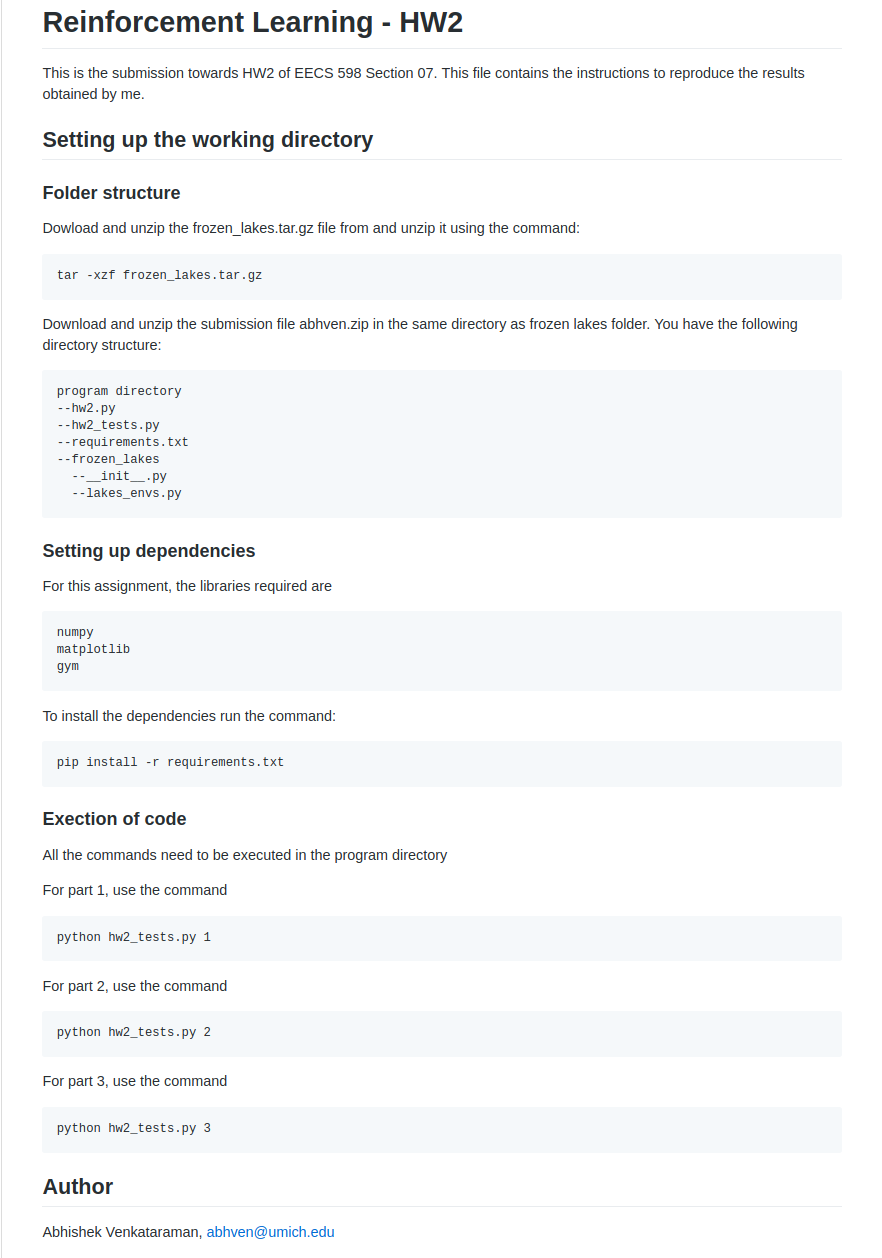
\includegraphics[width = 0.75\linewidth]{readme.png}
%		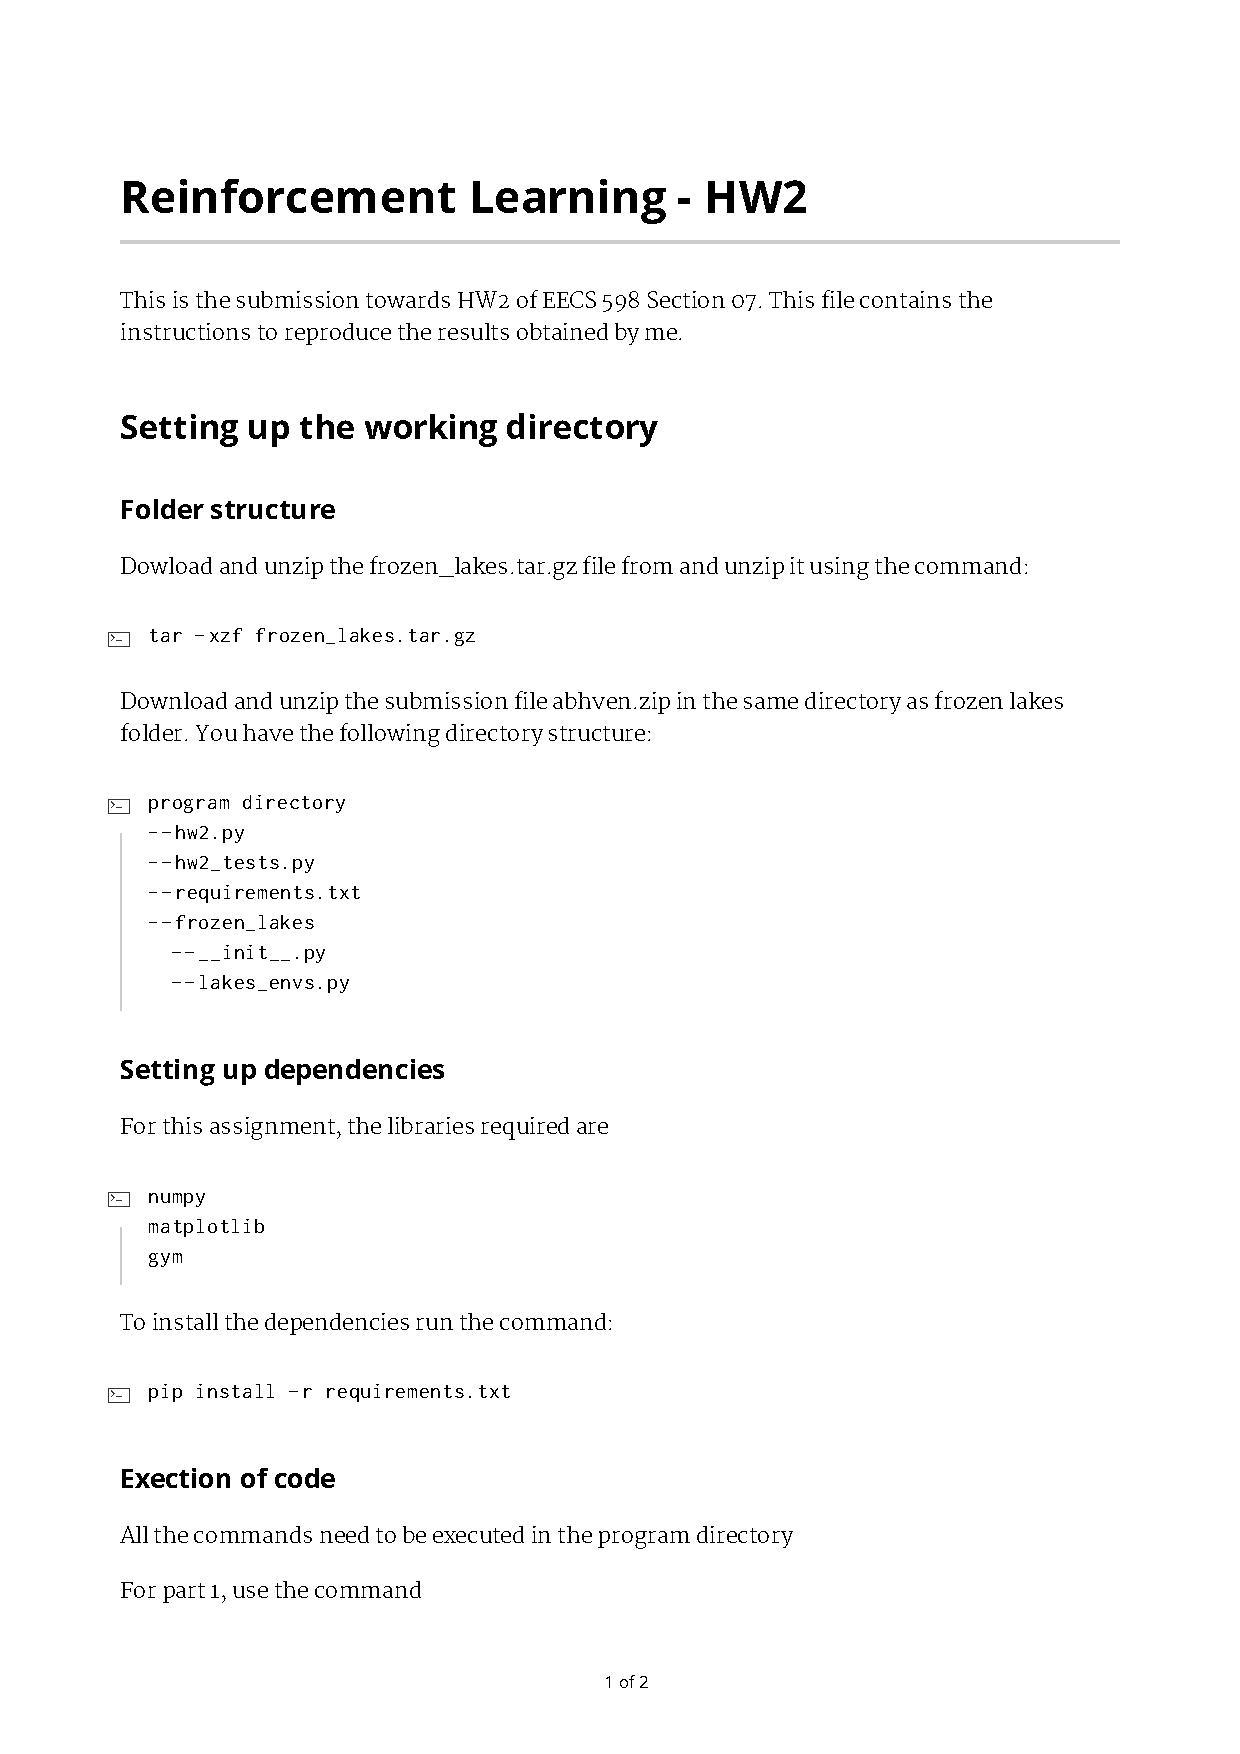
\includegraphics[page =1, width = 0.49\linewidth]{readme.pdf}
%		\includegraphics[page =2, width = 0.49\linewidth]{readme.pdf}
	\end{figure}
\end{itemize}

\end{problem}

\newpage	
\begin{problem} {5} Theory: Maximum-Likelihood estimate\\
\begin{proof}	
Given the MDP of n states, we want to find the transition probability,
\begin{align}
	p(S'=s'|S=s,A=a)	
	\nonumber
\end{align}	  
 
%\begin{align}
%L(p)=Pr(S'=s')\prod_{s\in S,a \in A}	p(S'=s'|S=s,A=a)
%\nonumber
%\end{align}	  
Let $n(s,a ->s')$ be the transition counts to state $s'$ from state $s$ by action $a$. Writing in terms of likelihood,
\begin{align}
L(p)=Pr(S'=s')\prod_{s\in S,a \in A}~\prod_{s'\in S'}	p(S'=s'|S=s,A=a)^{n(s,a ->s')}
\nonumber
\end{align}	 
Taking log form, 
\begin{align}
\log L(p)= \log Pr(S'=s') + \sum_{s\in S,a \in A, s'\in S'}	{n(s,a ->s')} \log p(s'|s,a) 
\nonumber
\end{align}
Taking the derivative,
\begin{align}
\dfrac{\partial \log L(p)}{\partial p(s'|s,a)}= \dfrac{n(s,a ->s')}{p(s'|s,a)} 
\nonumber
\end{align}
This is equal to 0 at $p(s'|s,a)$. Now we can get
\begin{align}
\dfrac{\hat n(s,a ->all)}{p(all|s,a)}= \dfrac{\hat n(s,a ->s')}{p(s'|s,a)} 
\nonumber\\
\therefore \dfrac{p(s'|s,a)}{p(all|s,a)}= \dfrac{\hat n(s,a ->s')}{\hat n(s,a ->all)} 
\nonumber
\end{align}
we know that ${p(all|s,a)} = 1$
\begin{align}
\therefore {p(s'|s,a)}= \dfrac{\hat n(s,a ->s')}{\hat n(s,a ->all)} 
\nonumber
\end{align}
 
\end{proof}	

\end{problem}

\begin{problem} {6} Theory: POMPDP belief state\\
\begin{figure}[h]
	\centering
	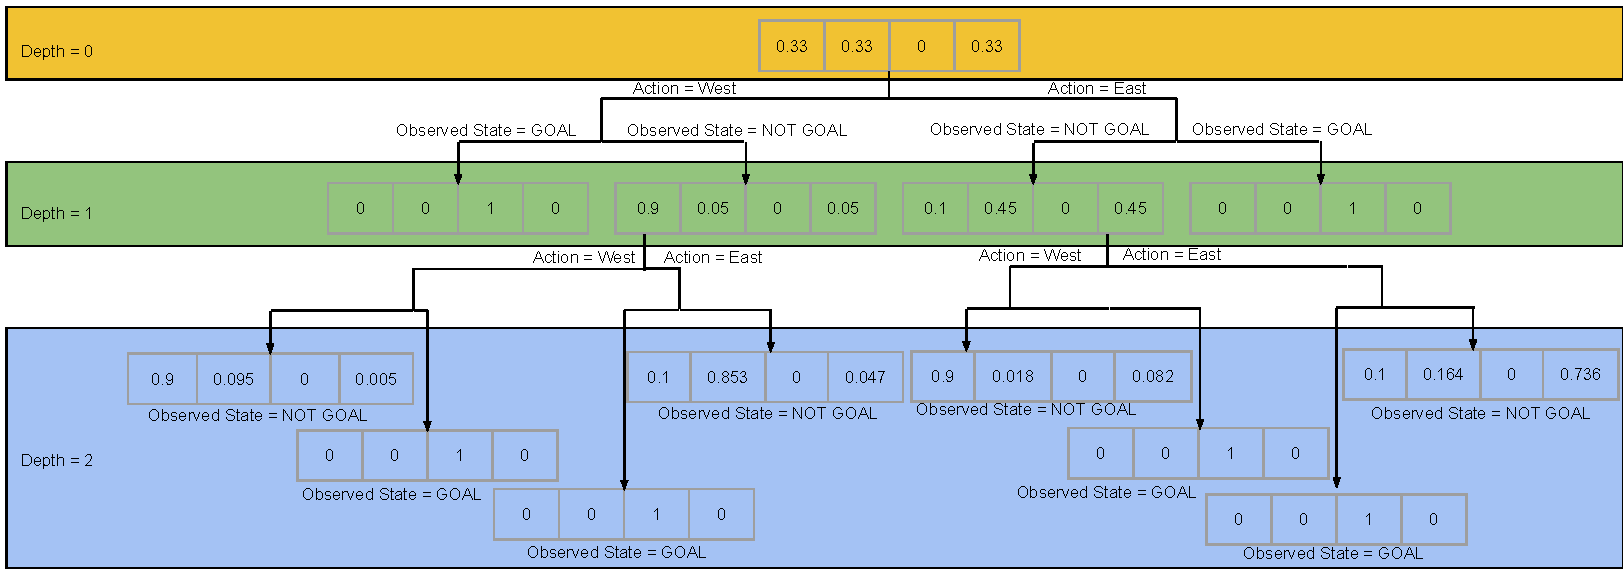
\includegraphics[width = 1\linewidth]{Belief_states.pdf}
	\end{figure}
\end{problem}
The belief state can be given by:
\begin{align}
b'(s')= \dfrac{O(s',a,o)\Sigma_{s\in S} T(s,a,s')b(s)}{Pr(o\vert a,b)}= \eta.O(s',a,o)\Sigma_{s\in S} T(s,a,s')b(s)
\nonumber
\end{align}
where $\eta$ is the normalization factor. Since the observation is only whether in goal state or not, 
\begin{align}
O(s', a , o) = &  \begin{cases}
0, ~\text{if}~ s' \in \{1,2,4\} ~ \mathtt{and} ~o = GOAL  \\
1, ~\text{if}~ s' \in \{1,2,4\} ~ \mathtt{and} ~o = NOT~ GOAL  \\
1, ~\text{if}~ s' \in \{3\} ~ \mathtt{and} ~o = GOAL  \\
0, ~\text{if}~ s' \in \{3\} ~ \mathtt{and} ~o = NOT ~GOAL  \\
\end{cases}
\nonumber
\end{align}
Clearly if we observe goal state, then belief state would take the value $[0,0,1,0]$. Hence the below calculations are shown only for non goal state observations.\\

\textbf{Depth = 1}\\
Action = West
\begin{align}
b'(1) &= \eta.1.\{T(1,W,1)b(1) + T(2,W,1)b(2)\}=\eta\{0.9\times0.33 + 0.9\times0.33\} &= 0.594\eta \nonumber\\
b'(2) &= \eta.1.\{T(1,W,2)b(1) \}=\eta 0.1\times0.33 &= 0.033\eta \nonumber\\
b'(3) & &=0 \nonumber\\
b'(4) &= \eta.1.\{T(4,W,4)b(1) \}=\eta 0.1\times0.33 &= 0.033\eta \nonumber\\
\nonumber
\end{align}
Solving $\Sigma_{s \in \{1,2,3,4\}} b'(s')=1$, belief state = $[ 0.9,0.05,0,
0.05]$ \\

\textit{Action = East}
\begin{align}
b'(1) &= \eta.1.\{T(1,E,1)b(1) + T(2,E,1)b(2)\}=\eta\{0.1\times0.33 + 0.1\times0.33\} &= 0.067\eta \nonumber\\
b'(2) &= \eta.1.\{T(1,E,2)b(1) \}=\eta 0.9\times0.33 &= 0.297\eta \nonumber\\
b'(3) & &=0 \nonumber\\
b'(4) &= \eta.1.\{T(4,E,4)b(1) \}=\eta 0.9\times0.33 &= 0.297\eta \nonumber\\
\nonumber
\end{align}
Solving $\Sigma_{s \in \{1,2,3,4\}} b'(s')=1$, belief state = $[ 0.1,0.45,0,
0.45]$ \\

\textbf{Depth = 2}\\
\textit{Depth 1 Action = West, Depth 2 Action = West}
\begin{align}
b'(1) &= \eta.1.\{T(1,W,1)b(1) + T(2,W,1)b(2)\}=\eta\{0.9\times0.9 + 0.9\times0.05\} &= 0.855\eta \nonumber\\
b'(2) &= \eta.1.\{T(1,W,2)b(1) \}=\eta 0.1\times0.9 &= 0.09\eta \nonumber\\
b'(3) & &=0 \nonumber\\
b'(4) &= \eta.1.\{T(4,W,4)b(1) \}=\eta 0.1\times0.05 &= 0.005\eta \nonumber\\
\nonumber
\end{align}
Solving $\Sigma_{s \in \{1,2,3,4\}} b'(s')=1$, belief state = $[ 0.9,0.095,0,
0.005]$ \\

\textit{Depth 1 Action = West, Depth 2 Action = East}
\begin{align}
b'(1) &= \eta.1.\{T(1,E,1)b(1) + T(2,E,1)b(2)\}=\eta\{0.1\times0.9 + 0.1\times0.05\} &= 0.095\eta \nonumber\\
b'(2) &= \eta.1.\{T(1,E,2)b(1) \}=\eta 0.9\times0.9 &= 0.81\eta \nonumber\\
b'(3) & &=0 \nonumber\\
b'(4) &= \eta.1.\{T(4,E,4)b(1) \}=\eta 0.9\times0.05 &= 0.045\eta \nonumber\\
\nonumber
\end{align}
Solving $\Sigma_{s \in \{1,2,3,4\}} b'(s')=1$, belief state = $[ 0.1,0.853,0,
0.047]$ \\

\textit{Depth 1 Action = East, Depth 2 Action = West}
\begin{align}
b'(1) &= \eta.1.\{T(1,W,1)b(1) + T(2,W,1)b(2)\}=\eta\{0.9\times0.1 + 0.9\times0.45\} &= 0.495\eta \nonumber\\
b'(2) &= \eta.1.\{T(1,W,2)b(1) \}=\eta 0.1\times0.1 &= 0.01\eta \nonumber\\
b'(3) & &=0 \nonumber\\
b'(4) &= \eta.1.\{T(4,W,4)b(1) \}=\eta 0.1\times0.45 &= 0.045\eta \nonumber\\
\nonumber
\end{align}
Solving $\Sigma_{s \in \{1,2,3,4\}} b'(s')=1$, belief state = $[ 0.9,0.018,0,
0.082]$ \\

\textit{Depth 1 Action = East, Depth 2 Action = East}
\begin{align}
b'(1) &= \eta.1.\{T(1,E,1)b(1) + T(2,E,1)b(2)\}=\eta\{0.1\times0.1 + 0.1\times0.45\} &= 0.055\eta \nonumber\\
b'(2) &= \eta.1.\{T(1,E,2)b(1) \}=\eta 0.9\times0.1 &= 0.09\eta \nonumber\\
b'(3) & &=0 \nonumber\\
b'(4) &= \eta.1.\{T(4,E,4)b(1) \}=\eta 0.9\times0.45 &= 0.405\eta \nonumber\\
\nonumber
\end{align}
Solving $\Sigma_{s \in \{1,2,3,4\}} b'(s')=1$, belief state = $[ 0.1,0.164,0,
0.736]$ \\

\begin{problem} {7} Theory: Optimum policy with fixed horizon\\

When the horizon to be 1, clearly, the 
\begin{align}
	\pi^*_1(s)= \argmax_a  R(s,a) \nonumber\\
	V_1(s)\coloneqq R(s,\pi_1(s)) ~~\forall s \in S
	\nonumber
\end{align}	
Now for horizon of 2 and 3, using $V_1(s)$,\\

Initialize $V_2(s) = 0 $  $\forall s \in S $\\
\textbf{loop} for all $ t \in \{2,3\}$ \\
\hspace*{10mm}\textbf{loop} for all $ s \in S$ \\
\hspace*{10mm}\hspace*{10mm} \textbf{loop} for all $ a \in A$\\
\hspace*{10mm}\hspace*{10mm}\hspace*{10mm} $Q_t^a(s) \coloneqq R(s,a) + \Sigma_{s' \in S} T(s,a,s') V_{t-1}(s') $\\
\hspace*{10mm}\hspace*{10mm} \textbf{end loop}\\
\hspace*{10mm}\hspace*{10mm} $V_t(s) \coloneqq \max_a Q^a_t(s)$\\
\hspace*{10mm} \textbf{end loop}\\
\textbf{end loop}\\

Hence the optimal policy with 3 steps look ahead can be given by :

\begin{align}
\pi^*(s)= \argmax_a \begin{bmatrix} R(s,a) + \Sigma_{s' \in S} T(s,a,s')V_3(s')     \end{bmatrix} \nonumber
\end{align}

\end{problem}


\begin{problem} {8} Meta\\
I feel that 1 week was quite a small time for this assignment. I understand the course is being taught for the first time, however, it was quite frustrating that there were so many changes in the HW. Also the additional time constraint and uncertainty made the assignment challenging. 

\begin{itemize}
	\item Prob 1 \& 2:It took a lot of time to try out the parameters. I would have spent around 10-12 hours for coding, debugging and fine tuning the parameters.
	\item Prob 3: The implementation was not too hard. I spent a total of 3 hours on this problem
	\item Prob 4: I spent around 4 hours on this problem. 1 hour was spend on understanding the use fo requirements.txt and tesing it on a another linux machine. The README.md took around 0.5 hours since I have never made one before. 2.5 hrs was spent towards manually testing the algorithm.
	\item Prob 5: I spent around 3 hours on this problem. Most of the time was spent in trying to understand the question. 
	\item Prob 6: I spent around 3 hours on this problem 
	\item Prob 7: I spent around 3 hours on this problem
	
\end{itemize}


\end{problem}


\end{document}